\documentclass[hyperref,12pt]{ctexart}
\graphicspath{{fig/}}
\usepackage{hyperref}
\usepackage{amssymb}
\usepackage{mathrsfs}
\usepackage{amsmath}
\usepackage{indentfirst}
\usepackage{graphicx,color}
\usepackage{xcolor}
\usepackage{listings}
\usepackage{booktabs}
\usepackage{tabularx}
\usepackage{longtable}
\usepackage{enumerate}
\usepackage{fontspec}
\usepackage{overpic} % 在图片上叠加TeX公式
\usepackage[numbers,sort&compress]{natbib}
\usepackage[toc,page]{appendix}
\hypersetup{colorlinks=false}
\usepackage{geometry}
\geometry{lmargin={3.08cm},rmargin={2.18cm},tmargin={2.54cm},bmargin={2.54cm}}
\pagestyle{plain}

\begin{document}
\thispagestyle{empty}
\begin{titlepage}
%%\vspace*{2cm}
  {\LARGE \raggedleft \textbf{关于高维问题的一些总结}}\\
%%  \vspace*{0.5cm}
  \rule{\linewidth}{1.5mm}
  \vskip 0.1in
  \begin{flushright}
  \textbf{专业: 概率统计}\\
  \textbf{姓名: 高涛}\\
  \end{flushright}

 \vspace*{\fill}
%%  \vspace*{10cm}

  {\Large
    \noindent {\textbf{2013年3月}\\
    \rule{\linewidth}{1mm}}
  }
\end{titlepage}
\clearpage


\begin{center}
\zihao{3}{\textbf{高维变量选择问题}}\\
\vskip 0.15in
\end{center}
\hrule
\vskip 0.1in
\textbf{摘要}\hspace*{1em}
本文将简单回顾各类高维变量选择方法,并简单分析它们的性质。\\
\textbf{关键词}\hspace*{1em} 变量选择;惩罚项
\vskip 0.1in
\hrule

\section{背景介绍}
以前的模型选择方法多基于AIC、BIC、RIC、MDL、FIC准则,但是模型自变量比较多时候,信息准则计算量过大而无能为力,而且选择模型不稳定。这些方法在面对高维问题时,多用来调参。其实模型选择的问题也就是变量选择的问题,它有以下几个目标:
\begin{enumerate}[(1)]
	\item 对于数据驱动模型来说,首先要预测准确?
	\item 模型具有可解释性,选择的变量具有实际的意义?
	\item 选择的模型比较稳定,数据的微小变动不会导致模型发生巨大变化;
	\item 估计量要有一致性;
	\item 模型选择过程计算复杂程度要低?
\end{enumerate}

基于penalty OLS即一种新的模型选择方法(变量选择)。最先获得成功的是Lasso方法,但Lasso在一定条件下不具有Oracle Property,于是Fan提出了SCAD,也给出了对于惩罚函数选择的更一般的研究框架—— 似然惩罚,并有“局部二次近似”算法。一般选择Tunning parameters用GCV方法。

所谓Oracle性质:若$A= \{i | \hat{\boldsymbol{\beta}} \neq 0\}$, $A$中元素个数小于总变量数,$A$表示不为0的系数,有
\begin{enumerate}[(1)]
	\item Sparsity:除了$A$中元素对应的估计系数$\hat{\boldsymbol{\beta_1}}$,其余的估计$\hat{\boldsymbol{\beta_2}} = \mathbf{0}$,即随着样本量趋向无穷,估计系数不为0的系数个数等于真实个数的概率为1。
	\item 真实参数$\sqrt{n}(\hat{\boldsymbol{\beta_1}} - \boldsymbol{\beta_1}) \rightarrow_L N(0, \boldsymbol{\Sigma})$,$\boldsymbol{\Sigma}$为真实参数模型参数的协方差。
\end{enumerate}
这种性质在Lehnmann的书中称作“superefficiency”。

\section{模型介绍}
现假定线性回归模型
\[
\mathbf{y} = \mathbf{X}\boldsymbol{\beta}
\]

其中$\mathbf{y}$是$n\times 1$向量,而$\mathbf{X}$是$n \times d$的矩阵,假定给了设计矩阵$\mathbf{X}$后$y_i$条件独立。不失一般性,假设设计矩阵$\mathbf{X}$列正交,于是OLS估计$\hat{\boldsymbol{\beta}} = \mathbf{X'y}$。此时另$\mathbf{z} = \mathbf{(X'X)^{-1}X'y} = \mathbf{X'y}, \hat{\mathbf{y}} = \mathbf{X(X'X)^{-1}X'y} = \mathbf{XX'y}$,则penalized OLS为:
\begin{equation}
\frac{1}{2}\|\mathbf{y} - \mathbf{X}\boldsymbol{\beta}\|^2 + \lambda\sum_{j = 1}^d p_j(|\beta_j|) = \frac{1}{2}\|\mathbf{y} -\hat{\mathbf{y}}\|^2 + \frac{1}{2}\sum^d_{j = 1}(z_j - \beta_j)^2 + \lambda\sum_{j = 1}^d p_j(|\beta_j|)
\end{equation}

其中penalty $_j(\cdot)$不必对每个$j$都相同,此处假设都相同,记为$p_{\lambda}(\cdot)$。最小化上式及等价于\textbf{最小化每个系数的估计},即只需考虑如下最小二乘问题:

\[
\frac{1}{2}(z - \theta)^2 + p_{\lambda}(|\theta|)
\]

\subsection{惩罚函数形式}
下面给出各种惩罚函数和相应的估计:
\begin{enumerate}[(1)]
	\item 对于hard thresholding penalty函数(Antoniadis, Fan, 1997):
	$$p_{\lambda}(|\theta|) = \lambda^2 - (|\theta| - \lambda)^2 I(|\theta| < \lambda)$$
	显然,这种惩罚项在$|\theta| > \lambda$时对$\theta$没有惩罚,小于时给予一定惩罚,获得解为
	$$\hat{\theta} = zI(|z| > \lambda)$$
	对应着best subset选择和逐步回归的估计。
	
	\item Lasso的L1惩罚:$p_{\lambda} = \lambda|\theta|$(Tibshiran 1996)。
	这种惩罚项可以看到对每一个系数$\theta$惩罚度是一样的,对应的解为
	$$\hat{\theta} = \text{sgn}(z)(|z| - \lambda)_{+}$$
	此种惩罚对应着soft thresholding rule(Donoho \& Johnstone 1994)。
	
	\item 岭回归为L2惩罚$p_{\lambda} = \lambda|\theta|^2$,同L1 类似,对每个系数的惩罚度相同,对应的解为
	$$\hat{\theta} = \frac{z}{1 + 2\lambda}$$
	\item Bridge Regression的一般化$p_{\lambda} = \lambda|\theta|^q$,Lasso和岭回归都是它的特殊情况,$q = 0$ 时,为OLS估计,其他值一般无显示解。当$q \rightarrow 0$时,岭回归又可以看做是L0惩罚$\lim_{q \rightarrow 0}\sum^d_{j = 1}|\theta|^q  = \sum^d_{j = 1}I(\theta \neq 0) $
	
	\item Nonnegative Garrote的惩罚为$p_{\lambda} = \lambda\frac{1}{|z|}|\theta|$,可以看到这种惩罚与$z$有关,换句话说,$z$大时对$\theta$惩罚小,$z$小时对$\theta$惩罚大,这与后续的Adaptive lasso比较相似,拥有Oracle性质?对应的解为
	$$\hat{\theta} = \text{sgn}(z)(z - \frac{\lambda}{|z|})_+$$
	
	\item Adaptive lasso的惩罚似乎是Nonnegative Garotte的一般化,同样对大的系数惩罚小,对小的系数惩罚大,具有自适应性,此时该种惩罚具有Oracle 性质,证明后续会附上:$p_{\lambda} = \lambda\frac{1}{|z|^r}|\theta|$,但是实际$r$的选择是调参得来的,其估计为:
	$$\hat{\theta} = \text{sgn}(z)(|z| - \frac{\lambda}{|z|^r})_+$$
	
	\item 另外,整合了L1和L2惩罚的elastic net惩罚为$p_{\lambda}(|\theta|) = \lambda_1|\theta| + \lambda_2|\theta|^2$,对应的估计为
	$$\hat{\theta} = \text{sgn}(z)(|z| - \frac{\lambda_1}{2})_+$$
	
	\item 具有很好Oracle性质的SCAD惩罚为
	\[
	p_{\lambda}(|\theta|) = \left\{\begin{array}{lr}
	\lambda|\theta|, & 0 \leq |\theta| < \lambda; \\
	-(|\theta|^2 - 2a\lambda|\theta| + \lambda^2)/(2(a - 1)), & \lambda \leq |\theta| < a \lambda; \\
	(a + 1)\lambda^2/2, & |\theta| \geq a\lambda
	\end{array}
	\right.
	\]
	常说的SCAD(smoothly clipped absolute deviation penalty)其实是该函数的导数$$p'_{\lambda}(|\theta|) = \lambda\{I(\theta < \lambda) + \frac{(a\lambda - \theta)_{+}}{(a - 1)\lambda}I(\theta > \lambda) \}, a >2, \theta > 0$$
	花括号中的项目降低了对大系数的惩罚,因为当$\beta > \lambda, a \geq 2$时,如果$a\lambda$比$\beta$小,那么对大系数就不惩罚了,如果比$\beta$ 大,手动计算下即可发现则由于$a$ 的作用使得$\lambda$变小了,此时对大系数惩罚就降低了。获得的估计为
	\[
	\hat{\theta}=\left\{\begin{array}{lr}
	\text{sgn}(z)(|z| - \lambda)_{+}, & |z| \leq 2\lambda; \\
	\{(a - 1)z - \text{sgn}(z)a\lambda\}/(a - 2), & 2\lambda < |z| \leq a \lambda; \\
	z, & |z| > a \lambda
	\end{array}
	\right.
	\]
	\item relaxed lasso对应的惩罚为$p_{\lambda}(|\theta|) = \phi\lambda|\theta|, \phi \in [0, 1]$。思想很简单,即由于lasso 估计的非零解有偏,为减轻这种偏差,先用lasso估计一遍,提取出来一组非零解,然后再用GCV法选取一次参数,在第一次提取出来的非零解变量上再得到一次lasso估计,对应的解为
	\[
	\hat{\theta} = \left\{\begin{array}{lr}
	z - \phi\lambda, & z > \lambda, \\
	0, & |z| \leq \lambda, \\
	z + \phi\lambda, & z < -\lambda
	\end{array}
	\right.
	\]	
\end{enumerate}

\subsection{惩罚函数性质}
Fan(2001)给出的一个好的惩罚函数应该具有如下性质:
\begin{enumerate}[(1)]
	\item 无偏性:未知参数真实值较大时,估计应几乎无偏。
	\item 稀疏性:有一个thresholding准则,自动将将较小的估计系数降至为0,以降低模型复杂度。
	\item 连续性:为避免预测模型的不稳定性,导出的估计应该是$z$ 的连续函数。
\end{enumerate}

上述第(2)条对于变量选择问题非常重要,这样可以大大降低模型复杂度,选取重要的变量。而无偏性则类似Oracle性质,最后的连续性为了稳定的需要,上述惩罚中Hard thresholding不满足连续性,估计的系数有跳跃,而lasso只会在协方差阵满足一些条件时才有这一致性(一般会有偏)。其余的SCAD、Adaptive lasso、elastic net等都有相似的性质,满足三个条件。

观察\[
\frac{1}{2}(z - \theta)^2 + p_{\lambda}(|\theta|)
\]
中的$p_{\lambda}(\cdot)$是一个$(0, \infty)$的非负非降可微函数,当$|\theta|\rightarrow \infty$时,函数趋近无穷,则上述最小的$\theta$ 会存在。下面给出满足三条件的充要条件(Antoniadis \& Fan, 2001):

若$p_{\lambda}(\cdot)$是一个$(0, \infty)$的非负非降可微函数,并且函数$-\theta - p'_{\lambda}(|\theta|)$在$(0, \infty)$时严格单峰函数,那么:
\begin{enumerate}[(1)]
	\item 原函数的OLS解存在,且$\hat{\theta}(z)$是关于$z$的奇函数。即$\hat{\theta}(-z) = -\hat{\theta}(z)$。
	\item 解有如下性质:
	\[
	\hat{\theta}(z) = \left\{\begin{array}{lr}
	0, & |z| \leq p_0 \\
	z - \text{sgn}(z)p'_{\lambda}(|\hat{\theta}(z)|), & |z| > p_0
	\end{array}
	\right.
	\]
	其中$p_0 = \text{min}_{\theta \geq 0}\{\theta + p'_{\lambda}(\theta)\}, |\hat{\theta}(z)| \leq |z|$。
	\item 若$p'_{\lambda}(\cdot)$是非增函数,那么当$|z| > p_0$ 时,有
	$$|z| - p_0 \leq |\hat{\theta}(z)| \leq |z| - p'_{\lambda}(|z|)$$
	\item 若$p'_{\lambda}(\theta)$在$(0, \infty)$上连续,那么解$\hat{\theta}(z)$是连续的当且仅当函数$\theta + p'_{\lambda}(\theta)$最小值在0 处达到。
	\item 若$|z| \rightarrow \infty, p'_{\lambda}(|z|) \rightarrow 0$,则有:
	$$\hat{\theta}(z) = z - p'_{\lambda}(|z|) + o(p'_{\lambda}(|z|))$$	
\end{enumerate}

\subsection{性质的理解}
\textbf{上述性质最为重要的是第二点的理解。}目标函数$\frac{1}{2}(z - \theta)^2 + p_{\lambda}(|\theta|)$的导数为$\theta + \text{sgn}(\theta)p'_{\lambda}(|\theta|)$,如果$|z| < \text{min}_{\theta > 0}\{\theta + p'_{\lambda}(\theta)\}$,那么导数就一直为正,目标函数只能在$\theta = 0$处取最小值;当$|z| > \text{min}_{\theta > 0}\{\theta + p'_{\lambda}(\theta)\}$时,那么此时$\theta = z - p'_{\lambda}(|\hat{\theta}|)$目标函数取得最小值,这样就有了一个阈值,即(2)中的$p_0$,将小于它的值系数压制为0,大于它的值则系数有一定的调整,这就实现了稀疏性。此时若想保证连续性,很显然$p_0 = \text{min}_{\theta \geq 0}\{\theta + p'_{\lambda}(\theta)\} = 0$即可,这也是\textbf{第四点的要求}。如果还要实现无偏性,那么对(2) 中的$p'_{\lambda}(|\hat{\theta}(z)|)$ 进行适当的设计,当$z$ 超过一定值,该导数为0即可有$\hat{\theta}(z) = z$。 此时这样的惩罚函数就满足了Fan(2001)提出的好惩罚函数的性质了!

而在第三点和第五点下,加一些条件绘制的出来的penalty曲线就是一种concave的图形了。比如$p'_{\lambda}(\theta)$非增且在$|z| \rightarrow \infty$时$p'_{\lambda}(|z|) \rightarrow 0$,而$p'_{\lambda}(z)$按第四点要求又是连续的,那么其实就是$p'_{\lambda}(\theta)$逐渐减少,最后趋于0。反映到图形上来,就是penalty 的斜率越来越小,最后变成平坦的。如下图\ref{scad}。

\begin{figure}[ht]
\centering
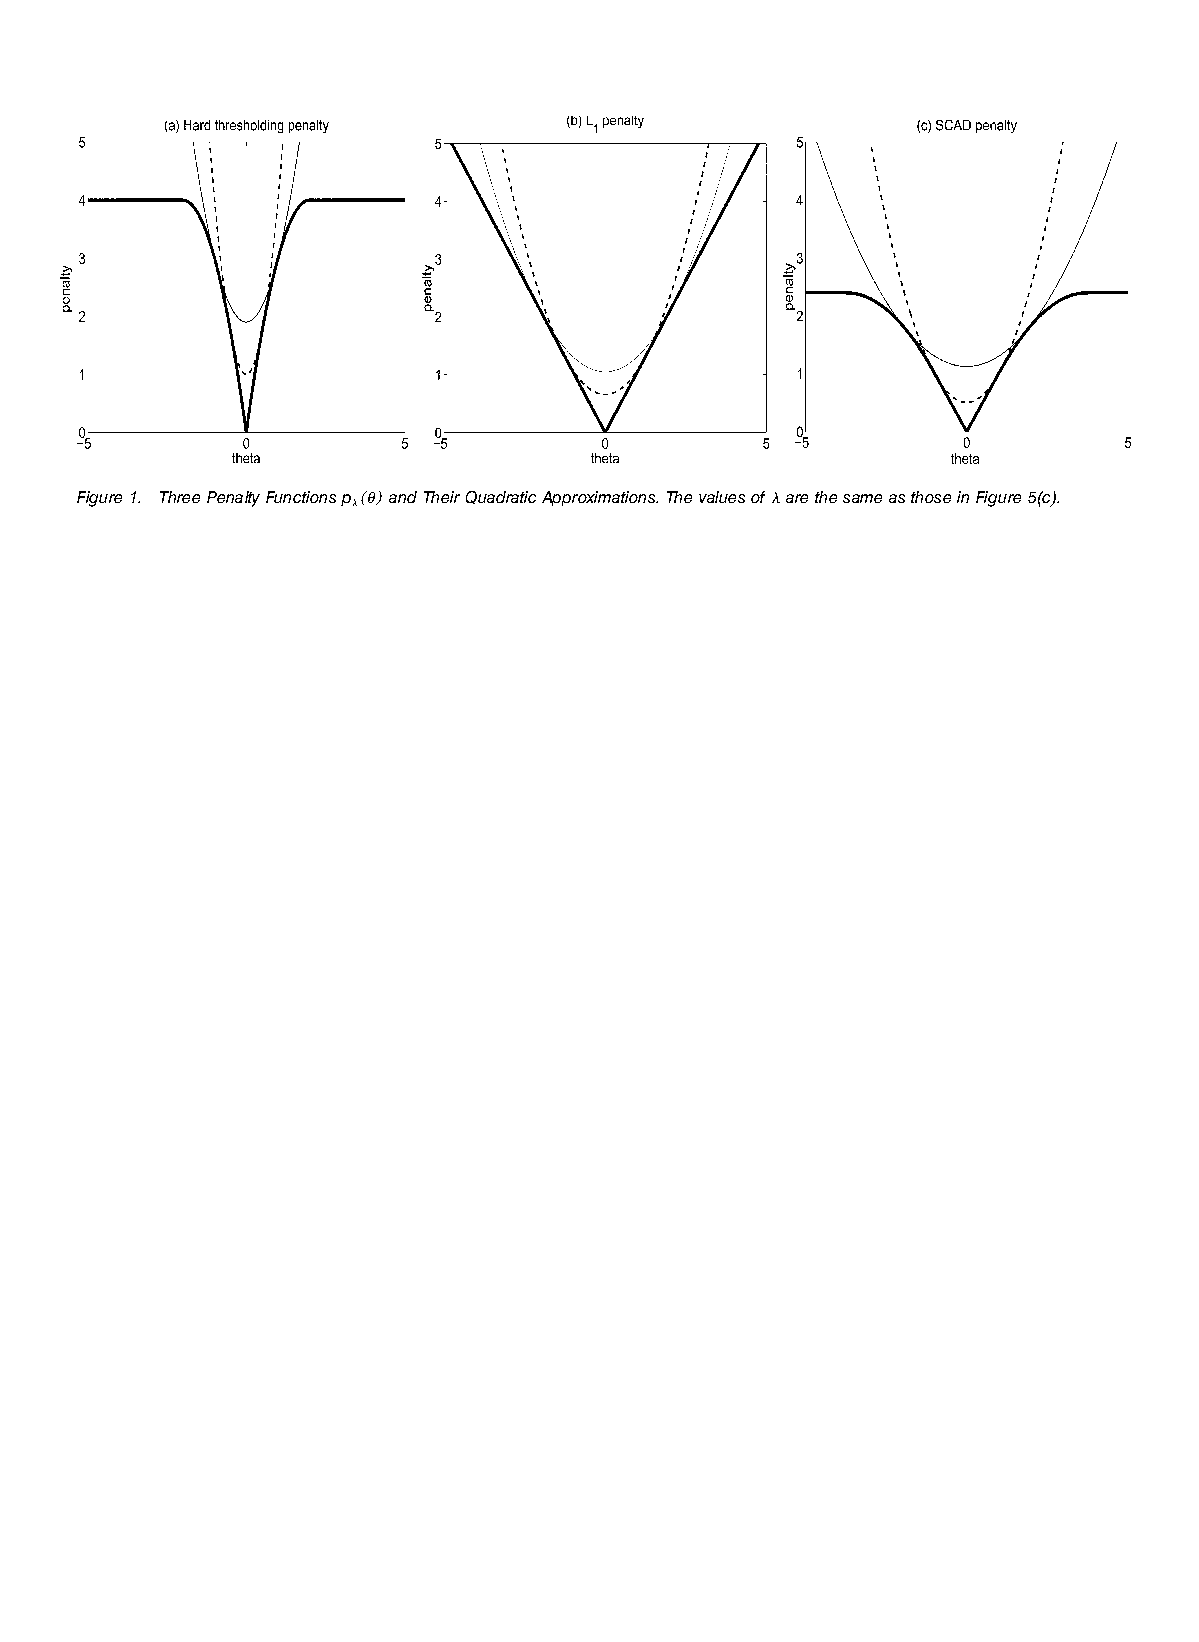
\includegraphics[width = 0.9\textwidth]{scad.pdf}
\caption{SCAD、LASSO、Hard Threshold的penalty导数$p'_{\lambda}(\theta)$的图形变化}\label{scad}
\end{figure}

Fan在2001年的文章上探讨penalty的性质与上述给出充要条件叙述方式不同,此处叙述的更为形象、易于理解。他直接从目标$\frac{1}{2}(z - \theta)^2 + p_{\lambda}(|\theta|)$的导数$\text{sgn}(\theta)\{|\theta| + p'_{\lambda}(\theta)\} - z$ 出发,为了要得到大的系数为无偏的,则只需要$p'_{\lambda}(\theta) = 0$即可。 而为了能够有变量选择作用,则对于某个$z$来说,如果$z$过小,则目标导数最小只能在$\theta$ 为0处取得,那么估计参数$\theta(z)$就直接为0,这种就感觉看起来好像已经知道了真实参数$\theta=0$一样。 而如果此时$z$ 适中,比$\min_{\theta > 0}\theta + p'_{\lambda}(\theta)$ 大,那么就可以估计的最小值就可以按照这种方法获取。换句话说,就是$\theta$ 与其penalty的斜率$p'_{\lambda}(\theta)$的平衡情况,真实的$\theta$ 很小时,罚的斜率大,使得$z$比罚的斜率小,那么此时估计的$\hat{\theta}$ 就可以直接认为是0了。因为真实的情况下,目标函数要想达到最小,面对很小的$z$ (OLS系数),影响可以忽略掉。这个时候真实的$\theta$ 应该是0才是。这种感觉好像是因为条件要求真实参数如此,但是其实又有种感觉像是提前知道了真实参数就该为0 一样,所以被称作“神谕(Oracle)”,表示理论与真实的某种相符合性。当$\theta$ 比较适中时,而$z$ 也算适中时,可以就取目标函数相应的最小值,算是给予本来的OLS 估计$z$ 一个惩罚。因此这个时候就需要penalty 的导数$p'_{\lambda}(\theta)$ 在0 附近比较大,起到阈值作用,使得“真实”的参数真的估计为0了,然后慢慢地降低这个阈值,使得“真实”的参数逐渐与OLS估计相合。


那么现在反过来看看Fan提出的SCAD方法,其实从名字就有了这个感觉——平滑削减绝对偏差罚函数。对于未被shrinkage为0的系数,当$\theta \leq \lambda$时,$p'_{\lambda}(\theta) = \lambda$,估计的系数就有了偏差,当$\lambda < \theta \leq a\lambda$时,估计系数会有一个比$\lambda$小的偏差$\frac{(a\lambda - \theta)_{+}}{a - 1}, a > 2$,当$\theta > a\lambda$时,估计的系数就没有偏差。因此SCAD满足上述三个性质,而且拥有Oracle性质。Hard thresholding、Nonnegative Garrote、Lasso、Adaptive Lasso、SCAD三者估计系数的图形如下图\ref{fig}。不过实际中,Lasso导致的这种偏差并不大,毕竟惩罚系数还是比较小的,很大的参数与真实的参数间就可以近似相等了。

\begin{figure}[ht]
\centering
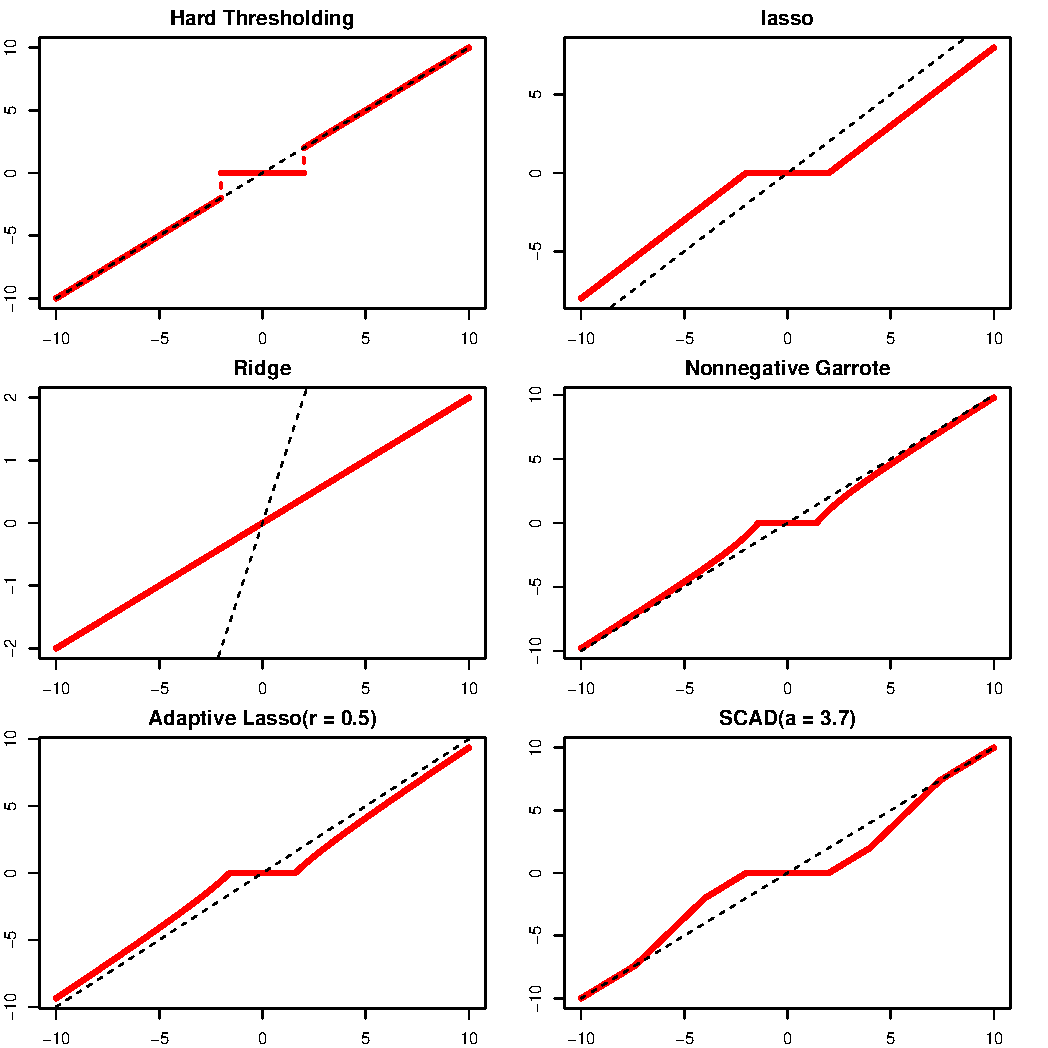
\includegraphics[width = 0.9\textwidth]{fig.pdf}
\caption{各种惩罚下所估计系数图形,注意此处$\lambda = 2$}\label{fig}
\end{figure}

从代数的角度来看这种加罚的最小二乘法,其实就是为了在原初的$\mathbb{R}^n$空间的子空间$W$中,再找一个子空间$W*$(限制条件导致,去掉一些小的系数),使得在子空间$W*$ 下对任意向量$\mathbf{Y}$ 的最佳逼近与在$W$中的最佳逼近在大的方面很相似(大的系数)。当然从似然的角度来看广义线性回归又有所不同了,损失函数不再是L2损失了。不过上述这种空间逼近的思维还是非常重要的,因为降维也就是一种空间近似。

在Fan最近的文章中(2012),提出了folded concave penalty为$P_{\lambda}(|t|) = P_{a, \lambda}(|t|)$,要求满足的条件其实与SCAD 是很相似:
\begin{itemize}
  \item $P_{\lambda}(t)$在$t \in [0, \infty)$上增加且是凹的(concave);
  \item $P_{\lambda}(t)$在$t \in (0, \infty)$上可微,且$P'_{\lambda}(0) = P'_{\lambda}(0+) \geq a_1 \lambda$;
  \item 当$t \in (0, a_2 \lambda]$时,$P'_{\lambda}(t) \geq a_1 \lambda$ ;
  \item 当$t \in [a \lambda, )$且$a > a_2$时,$P'_{\lambda}(t) \geq a_1 \lambda = 0$。
\end{itemize}

这个条件就是要求penalty成为一种折叠式的concave函数了。SCAD是$a_1 = a_2 = 1$的特殊情况,而MCP(zhang 2010a)是$a_1 = 1 - a^{-1}, a_2 = 1$的特殊情况,它的罚函数的导数为$P'_{\lambda}(t) = (\lambda - \frac{t}{a})_{+}$。folded concave penalty的图形如下图\ref{scad1}

\begin{figure}[ht]
\centering
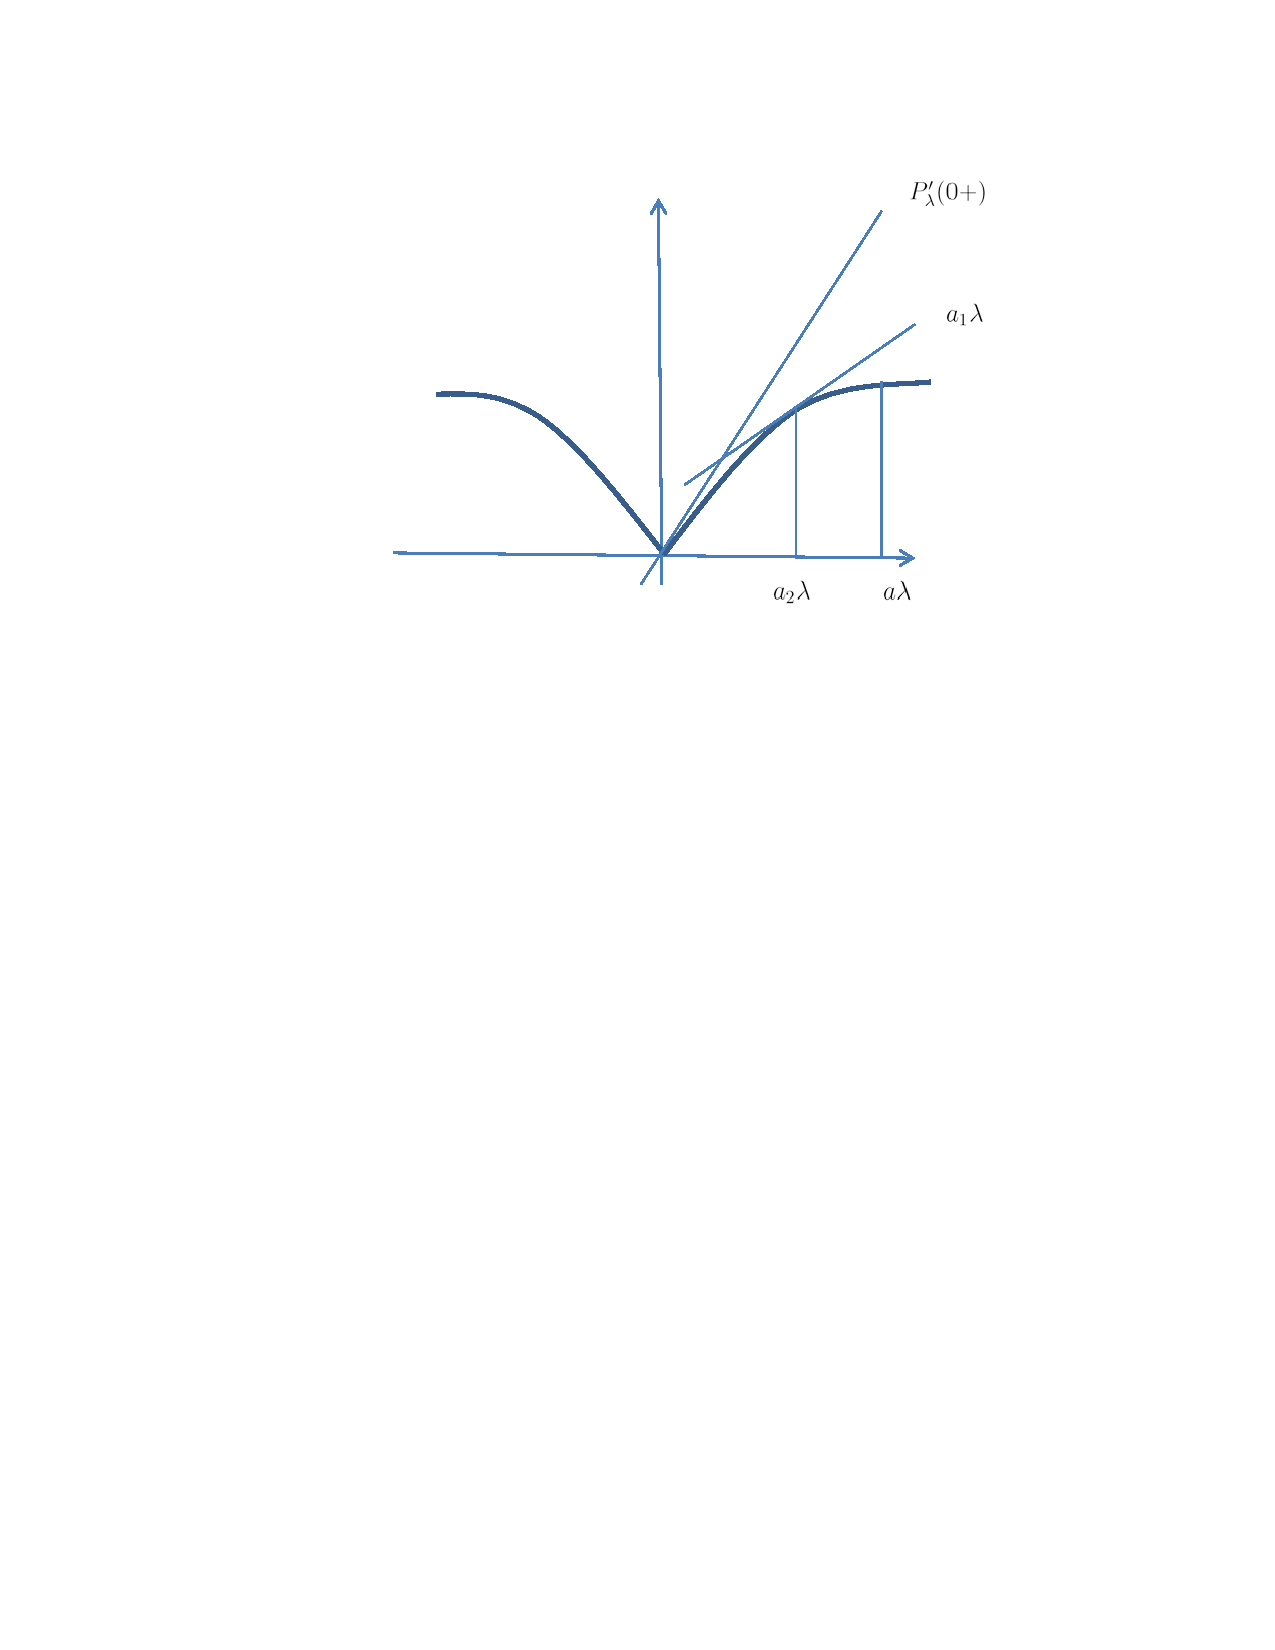
\includegraphics[width = 0.9\textwidth]{scad1.pdf}
\caption{general folded concave penalty的图形性质}\label{scad1}
\end{figure}



\section{收敛速度和Oracle性质}
\subsubsection{惩罚似然估计}
上述都是在$\mathbf{X}$列正交的情况讨论,一般化到广义线性模型上,那么将似然函数与惩罚项结合起来也相应的会具有上述性质。一般化的讨论框架为:

假定数据$\{\mathbf{x}_i, y_i\}$、 $\mathbf{x_i}$已知时,$y_i$ 有密度函数$f_i(g(\mathbf{x}_i^T\boldsymbol{\beta}, y_i))$,其中$g$是广义线性模型中的联结函数,$l_i=\text{log}f_i$表示$y_i$ 的对数似然函数,则惩罚最大似然估计的数学表达式为
\[
\text{max}_{\boldsymbol{\beta}}\quad \sum^n_{i = 1}l_i(g(\mathbf{x}_i^T\boldsymbol{\beta}), y_i) - n\sum_{j=1}^d p_{\lambda}(|\beta_j|)
\]
等价于
$\text{min}_{\boldsymbol{\beta}} -\sum^n_{i = 1}l_i(g(\mathbf{x}_i^T\boldsymbol{\beta}), y_i) + n\sum_{j=1}^d p_{\lambda}(|\beta_j|)$

\subsubsection{估计的渐进性质}
在之前的讨论中,我们希望惩罚后所得的估计具有稀疏性。但是稀疏性此时只是一个概念性,更具体地,我们希望能保证估计的非零系数个数以概率为1趋向于真实的非零个数,这样才能说估计的模型比较可靠,不会少选重要变量或多选无用的变量。同时,我们还希望知道估计系数的收敛速度,这样才好设计算法,评价算法的好坏。对于最基本的似然估计,我们知道他们有非常良好的性质,现在加入了惩罚项,那么惩罚项需要一些什么样的条件性质也可以获取非常好的理论性质呢?

在非凹惩罚似然函数中,假设真实参数为
\[
\boldsymbol{\beta}_0 = (\beta_{10},\ldots,\beta_{d0})^T =(\boldsymbol{\beta}_{10}^T, \boldsymbol{\beta}_{20}^T)
\]
并假设$\boldsymbol{\beta}_{20} = \mathbf{0}$。下面我们要证明的一个事情是惩罚似然估计的收敛速度为
\[
O_p(n^{-1/2} + a_n)
\]
其中,$a_n = \text{max}\{p'_{\lambda_n}(|\beta_{j0}|): \beta_{j0} \neq 0\}$。直观上来说,如果$\hat{\boldsymbol{\beta}}_{10}$是无偏估计,那么$\hat{\boldsymbol{\beta}}_{10}$的协方差阵即Fisher信息阵的倒数$I^{-1}(\boldsymbol{\beta}_{10})$,为0的系数的信息量仍然是0。 当然大样本来说,只要做到渐进无偏估计就已经足够了。当$\lambda_n \rightarrow 0$,我们就有了$\sqrt{n}$收敛速度的估计。下面是Fan(2001)的证明思路。

由于Fan是做Local出身,在非参方面有很深的造诣,因此他的证明也多是这种Local的思路。在证明收敛速度的时候,他先会根据目标收敛速度构造一个Local Maximizer 出来,然后利用泰勒展开证明收敛速度。不仅在SCAD 这篇文章中,以后的一些文章中证明收敛速度貌似基本都是这个技法,因此熟悉这个方法还是很重要的。下面通过一个定理的证明来熟悉这种证明技巧。由于涉及到极大似然估计问题,要极大似然估计的渐进正态性,需要满足一些正则条件(Lehmann TPS第二版P443和P462)。

\begin{enumerate}[(A)]
\item 观测点$\mathbf{V}_i$是独立同分布的,且概率密度函数$f(\mathbf{V}, \boldsymbol{\beta})$有共同的支集,模型可识别参数空间$\Omega$某个开子集$\omega$包含真参数$\boldsymbol{\beta}$,并是其内点。并且$f(\mathbf{V}, \boldsymbol{\beta})$三阶偏导对该开子集中的任何参数都存在。

\item 一阶和二阶对数偏导满足等式,以Cramer正则族一样
\[
E_{\boldsymbol{\beta}}\Big[ \frac{\partial \text{log}f(\mathbf{V}, \boldsymbol{\beta})}{\partial \beta_j}\Big] =  0, \quad j = 1, 2, \ldots, d
\]
以及
\[
\begin{split}
\mathbf{I}_{jk}(\boldsymbol{\beta}) = & E_{\boldsymbol{\beta}}\Big[ \frac{\partial}{\partial \beta_j} f(\mathbf{V}, \boldsymbol{\beta})\frac{\partial}{\partial \beta_k} f(\mathbf{V}, \boldsymbol{\beta})\Big] \\
= & E_{\boldsymbol{\beta}}\Big[- \frac{\partial^2 }{\partial \beta_j \partial \beta_k} \text{log}f(\mathbf{V}, \boldsymbol{\beta})\Big]
\end{split}
\]

\item Fisher信息阵在$\boldsymbol{\beta} = \boldsymbol{\beta}_0$ 处有限且正定。
\[
\mathbf{I}(\boldsymbol{\beta}) = E \Big\{ \Big[\frac{\partial}{\partial \boldsymbol{\beta}} \text{log}f(\mathbf{V}, \boldsymbol{\beta})\Big]\Big[\frac{\partial}{\partial \boldsymbol{\beta}} \text{log}f(\mathbf{V}, \boldsymbol{\beta})\Big]^T\Big\}
\]

\item 对于$\boldsymbol{\beta} \in \omega$的三阶偏导存在一个函数$M_{jkl}$使得
\[
|\frac{\partial}{\partial \beta_j \partial \beta_k \partial \beta_l} \text{log}f(\mathbf{V}, \boldsymbol{\beta})| \leq M_{jkl}
\]

其中$m_{jkl} = E_{\boldsymbol{\beta}_0}[M_{jkl}(\mathbf{V})] < \infty$。
\end{enumerate}

\textbf{定理1} \quad 一列独立同分布的观测$\mathbf{V}_1, \ldots, \mathbf{V}_n$,有密度函数$f(\mathbf{V}, \boldsymbol{\beta})$,满足上述正则条件,并且如果$\text{max}\{|p''_{\lambda_n}(\beta_{j0})|:\beta_{j0} \neq 0 \} \rightarrow 0$,则存在一个惩罚似然函数$Q(\boldsymbol{\beta}) = L(\boldsymbol{\beta}) - n\sum^d_{j = 1}p_{\lambda_n}(|\beta_j|)$ 局部最大值$\hat{\boldsymbol{\beta}}$满足$\| \hat{\boldsymbol{\beta}} - \boldsymbol{\beta}\| = O_p(n^{-1/2} + a_n)$,其中,$a_n = \text{max}\{p'_{\lambda_n}(|\beta_{j0}|): \beta_{j0} \neq 0\}$。

下面阐述Fan的证明收敛速度的一般思路。

\textbf{证明} 令$\alpha_n = n^{-1/2} + a_n$,首先构造一个存在局部极大值的依概率有界形式:对于任意$\epsilon > 0$,存在一个足够大的常数$C$使得
\[
P\Big\{\text{sup}_{\|\mathbf{u}\| = C} Q(\boldsymbol{\beta}_0 + \alpha_n \mathbf{u}) < Q(\boldsymbol{\beta}_0)\Big\} \geq 1 - \epsilon
\]

这个要求就使得在球域$\{\boldsymbol{\beta}_0 + \alpha_n \mathbf{u} : \mathbf{u}\| \leq C \}$中至少以概率为$1 - \epsilon$地存在局部极大值有$\| \hat{\boldsymbol{\beta}} - \boldsymbol{\beta}\| = O_p(\alpha_n)$。由于$p_{\lambda_n}(0) = 0$,因此有如下不等式收敛即可
\[
\begin{split}
D_n(\mathbf{u}) = & Q(\boldsymbol{\beta}_0 + \alpha_n \mathbf{u}) - Q(\boldsymbol{\beta}_0) \\
\leq & L(\boldsymbol{\beta}_0 + \alpha_n \mathbf{u}) - L(\boldsymbol{\beta}_0)- n\sum^s_{j = 1}\{p_{\lambda_n}(|\beta_{j0} + \alpha_n u_j|) - p_{\lambda_n}(|\beta_{j0}|)\}
\end{split}
\]
其中s是非零的参数个数,$s < d$,故不等式成立。下面进行泰勒展开有
\[
\begin{split}
D_n(\mathbf{u}) \leq & \alpha_n L'(\boldsymbol{\beta}_0)^T \mathbf{u} - \frac{1}{2}\mathbf{u}^TI(\boldsymbol{\beta}_0)\mathbf{u} n \alpha_n^2\{1 + o_p(1)\} \\
& - \sum_{j = 1}^s[n\alpha_n p'_{\lambda_n}(|\beta_{j0}|)\text{sgn}(\beta_{j0})u)j \\
& + n\alpha_n^2p''_{\lambda_n}u_j^2\{1 + o(1)\}
]
\end{split}
\]

注意$n^{-1/2}L'(\boldsymbol{\beta}_0) = O_p(1)$,因此上不等式右边的第一项阶数为$O_p(n^{1/2}\alpha_n) = O_p(n\alpha_n^2)$。 当选择足够大的$C$ 时,第二项一致控制了第一项,同理,第三项也会被第二项给控制,均当$\|\mathbf{u}\| = C$时。因此最初构造的局部极大值的概率不等式(依概率有界)成立。

上述的证明可以看到并不困难,只需要了解了证明速率的方式即可以。下面还有一个比较重要的性质——Oracle性质。此处不再证明,思想都是在给定条件下,泰勒展开后有相应的收敛速度控制,获得相应的渐进估计。

简要叙述Oracle性质即:当密度函数$f(\mathbf{V}, \boldsymbol{\beta})$满足上述正则条件,并且惩罚函数$p_{\lambda_n}(|\theta|)$满足条件
$$\liminf_{n \rightarrow \infty}\liminf_{\theta \rightarrow 0+}p'_{\lambda_n}(\theta)/ \lambda_n >0$$

当?$\lambda_n \rightarrow 0$,并且$\sqrt{n}\lambda_n \rightarrow \infty$,那么就有概率趋近于1的收敛速度为$\sqrt{n}$ 的局部最大化算子$\hat{\boldsymbol{\beta}} = \binom{\boldsymbol{\beta}_1}{\boldsymbol{\beta}_2}$满足:
\begin{enumerate}[(a)]
\item 稀疏性:$\boldsymbol{\beta}_2= \mathbf{0}$
\item 渐进正态性:$\sqrt{n}(\hat{\boldsymbol{\beta}}_1 - \boldsymbol{\beta}_{10}) \rightarrow N(\mathbf{0}, I_1(\boldsymbol{\beta}_{10})^{-1})$
\end{enumerate}


\section{算法}
\subsection{SCAD相关算法}
\subsubsection{Local Quadratic Approximation(LQA)}
既然是Fan提出的SCAD,当然是其熟悉的方法——local逼近法。2001年还没有最小角回归,即使有也没法解决他这个concave的惩罚函数。由于L1、hard thresholding和SCAD惩罚函数在0点奇异,且二阶导都不连续,但是还是可以利用一些技法通过二次函数来局部近似。Fan对于基于似然函数罚形式的问题,提出了通用的local quadratic approximation。方法很简单,首先假设初始值$\boldsymbol{\beta_0}$非常接近于最小值,
\textbf{如果某个$\beta_{j0}$非常接近于0,那么就设定$\hat{\beta}_j = 0$},否则$\beta_j \neq 0$ 的话,就用一个线性函数来逼近penalty的导数:
\[
[p_{\lambda}(|\beta_j|)]' = p'_{\lambda}(|\beta_j|)\text{sgn}(\beta_j) \approx \frac{p'_{\lambda}(|\beta_{j0}|)}{|\beta_{j0}|}\beta_j, \beta_{j0} \approx \beta_j
\]
对penalty做二阶泰勒展开,然后稍微做点运算即有
\[
\begin{split}
p_{\lambda}(|\beta_j|) \approx & p_{\lambda}(|\beta_{j0}|) + \frac{p'_{\lambda}(|\beta_{j0}|)}{\beta_{j0}}(\beta_j - \beta_{j0}) +  \frac{1}{2}\{\frac{p'_{\lambda}(|\beta_{j0}|)}{\beta_{j0}}\}(\beta_j - \beta_{j0})^2 \\
= & p_{\lambda}(|\beta_{j0}|) + \frac{1}{2}\{\frac{p'_{\lambda}(|\beta_{j0}|)}{\beta_{j0}}\}(\beta_j^2 - \beta_{j0}^2), \beta_j \approx \beta_{j0}
\end{split}
\]

然后对于整体目标函数$\ell(\boldsymbol{\beta})+ n \sum^d_{j = 1}p_{\lambda}(|\beta_j|)$ 做二阶泰勒展开(似然和最小二乘等的目标都可看做一种损失函数$\ell(\boldsymbol{\beta})$),就可以获取一个显示的解。

也可迭代求解,其中初始的$\boldsymbol{\beta}^{(0)}$是未加惩罚项的最大似然估计。
\[
\boldsymbol{\beta}^{(k+1)} = \text{arg\,max}\Big\{\sum^n_{i = 1} \ell_i(\boldsymbol{\beta)} - n \sum^p_{j = 1}\frac{p'_{\lambda}(|\beta_j^{(k)}|)}{2|\beta_j^{(k)}|}\beta_j^2\Big\}
\]
不过此时的假设依赖于初始值,需要初始点选的比较好,因此还是需要少量迭代(迭代步数很少时可看做一个好的one-step 估计,MLE 可以看做是一个one-step估计)。 效果还不错,相对之前不可计算此时计算速度快了许多,但是一个主要的不足就是一旦系数被压缩为0 后,就会停留在0点,也就是不会再选入模型了(类似逐步向后回归),而且依赖于初始点的选择。(这个是极大似然估计的通用方式)。

另外,由于上述假设\textbf{如果某个$\beta_{j0}$非常接近于0,那么就设定$\hat{\beta}_j = 0$},这容易导致删除点,一旦删除就无法在选入,因此还提出了个扰动LQA,但是效果还是一般啦。
\[
\boldsymbol{\beta}^{(k+1)} = \text{arg\,max}\Big\{\sum^n_{i = 1} \ell_i(\boldsymbol{\beta)} - n \sum^p_{j = 1}\frac{p'_{\lambda}(|\beta_j^{(k)}|)}{2\{|\beta_j^{(k)}| + \tau_0 \}}\beta_j^2\Big\}
\]
\subsubsection{Local Linear Approximation(LLA)}
Zou和Li(2008)提出one-step LQA无法获取稀疏解。并且由于容易犯与逐步向前回归一样的局部最优解(剔除了就无法再进入了),因此提出LLA。其实LLA真的很简单,就是用泰勒展开到一阶,而不展开到二阶。于是
\[
p_{\lambda}(|\beta_j|) \approx p_{\lambda}(|\beta_j^{(0)}|) + p'_{\lambda}(|\beta_j^{(0)}|)(|\beta_j| - |\beta_j^{(0)}|), \beta_j \approx \beta_j^{(0)}
\]

那么上述的迭代求解就变成了
\[
\boldsymbol{\beta}^{(k+1)} = \text{arg\,max}\Big\{\sum^n_{i = 1} \ell_i(\boldsymbol{\beta)} - n \sum^p_{j = 1}p'_{\lambda}(|\beta_j^{(k)}|)\beta_j\Big\}
\]

但是这个小小的变化为什么等了这么久才等来,本可以用一阶展开而不需要用二阶展开,按Fan 自己的说法是,2001 年时候Lasso的性质还没完全弄清楚,还没有非常有效的算法来解决。因此一阶展开,无法直接来解决$|\beta_j|$ 问题,而对于$\beta_j^2$问题,早就有了ridge regression,有加权OLS 方法。但这造成的问题是,其实LQA在这种迭代寻找$\beta_j^{(k)}$是一种岭回归问题,无法进行变量选择,因此结果不是很稳定,而且效果也不太好。所以当时Fan当时没用一阶展开,而是用了二阶展开来获取实际的结果。虽然Zou用LLA这么一小小的变换,但是使得one-step 估计都是sparse的,其实就变成了L1惩罚了。二阶到一阶展开,L2 问题变成了L1问题。于是只需要用LASSO类型方法来计算就可以了。Zou提出来的使用修正的LARS算法来解决两种类型penalty问题
\begin{itemize}
  \item $p_{\lambda}(t) = \lambda p(t), p'(t) > 0$,比如Bridge penalties等
  \item SCAD类型惩罚,无法将正则参数与penalty分开。
\end{itemize}

LLA的one-step estimator,用OLS或者MLE做最初的估计,然后在一步的估计获得的估计能够保证连续性,需要的条件相比Fan提出来的更弱,Fan需要最小值在0 处获得,而LLA只需要保证penalty的导数$p'_{\lambda}(|\theta|)$在$|\theta|>0$时连续就好了。


LLA是最优的convex minorization-maximization(MM)算法。注意,次数不是minimum,而是minorization,相差的尽可能地小么?MM算法是EM算法的扩展啊?
当正则参数选择的比较合适的时候


\subsubsection{Iterative(multiple) LLA}

\subsection{最小角回归(LARS)}

\subsection{坐标速降(CD)算法}
现在Lasso类问题的计算最快的方法(Friedman,2007)。思想描述起来十分简单,就是,与根据不断变化方向的梯度方法不同,CD是一种固定一些维度(坐标轴)然后不断下降得到局部最优解的方法,此时求解最小值其实都可以不用求导了。具体描述如待估参数共有$p$个,先固定住其中$p - 1$ 个,然后估计目标函数最小值时剩余参数,反复迭代直到所有的待估参数都收敛。这种方法速度非常快,但是要保证lasso 类解获得全局最优解,则需要满足几个条件,考虑目标函数
\[
f(\beta_1, \ldots, \beta_p) = g(\beta_1, \ldots, \beta_p) + \sum_{j = 1}^p h_j(\beta_j)
\]
CD收敛到全局最优的条件为:
\begin{itemize}
\item $g(\cdot)$是可微的凸函数;
\item $h_j(\beta_j)$是凸函数;
\item $\beta_j$可以是向量,但是$\beta_j$与$\beta_k$间不能有重叠的元素。比如$\sum_{j = 1}^p h_j(\beta_j) = \lambda \sum_i|\beta_i - \beta_{i - 1}|$ 就不行。
\end{itemize}

\section{Lasso相关问题的理解}
\subsection{从Bayes角度来看惩罚项}


\subsection{两步或多步估计(Adaptive Lasso的理解)}
Lasso估计的复杂度为$O(np\min(n, p))$,当$p \gg n$时,lasso就是线性复杂度了。对于lasso型估计,我们希望上述三个良好性质,但是lasso 一方面估计的参数会有偏,另外还有可能会误选变量。不误选变量,此时需要满足假设——非代表性条件(irrpresentable condition):$K$表示有关联变量集,$N$ 表示无关变量集
\[
\|\mathbf{X}^T_N \mathbf{X}_K(\mathbf{X}_K^T \mathbf{X}_K)^{-1} \text{sign}(\beta_K)\|_{\infty} <  1 \rightarrow
\text{max}_{j \in N}\|\mathbf{X}_j^N \mathbf{X}_K(\mathbf{X}_K^T\mathbf{X}_K)^{-1}\|_1 < 1
\]

直观来说就是$\mathbf{X}_N$这些重要变量与$\mathbf{X}_K$无关变量相关性不能太高,否则就会导致lasso筛选变量失败。这个条件还是比较严格的,对整体相关性来说有些过强了。

另外,Peter B\"{u}hlmann也提出了一个与非代表性条件接近,但是稍弱且解释性差点的假设(06年)——邻居稳定性条件(neighborhood stability condition)。该条件从图模型角度出发来构造。直观理解就是需要保证筛选变量间邻居变量的稳定性。但是这个条件是充分、几乎必要条件。

当然在更弱的假设下,lasso估计可以有更好的表现,可以达到$\|\hat{\beta}(\lambda) - \beta\|_q = o_p(1), q \in \{1, 2\}$,此处是小$o_p$而非大$O_p$,这个一致性已经非常强了。也就是说,之前达到的$O_p(1)$还不够,惩罚的还不够,lasso估计太松,使得包含真是模型的概率很容易趋近于1。换个角度说,根据MSE(prediction optimal)调的lasso估计模型过大过松,筛选变量还是多了。因此就出现了一些多步估计,加强惩罚,使得lasso估计更稀疏,而且保证一致性,这几种估计代表性有:LARS-OLS,relaxed lasso,adaptive lasso。都是为了降低估计的bias,使得估计更稀疏。

从更深层次来说,Lasso由于相同程度的压缩参数,当真实参数较大时,要想降低Lasso估计的bias,那么就还必须要对惩罚的收敛到0的速度做一些条件的限制,而对于SCAD等concave的penalty,由于满足Fan 之前提出的那些适应性的条件,对于惩罚并没有这些限制条件,很多性质获取都会更加直接。不过由于LLA算法的缘故,转化为L1问题,实际运算还是需要对设计阵$\mathbf{X}$做一些限制才行。(比如Compress sensing中的RIP条件。)

不过这几种估计都是one-step估计,如果需要更紧,还可以扩展到multi-step估计上来。这样惩罚更大,更加sparse。比如Peter B\"{u}hlmann 提的multi-step adaptive lasso,
\[
\lambda^{(k)}\sum^p_{j = 1}w_j^{(k-1)}|\beta_j|,\quad w_j^{(k)} = \frac{1}{|\beta^{(k-1)}(\lambda^{(k-1)})_j|}, w^{(0)}=1
\]
当$k=1$就是lasso,当$k=2$就是adaptive lasso。

不过这还只是理论上的结果,现实中,如果真实的active variables比较少时,多步估计会有比较好的表现,false positive rate比较小,但若真是的active variables 比较多时,很显然也不符合multi-step估计的目标,反而会导致multi-step 估计不如one-step估计了。(理论上讲应该是收敛的才对,不过由于实际惩罚参数的调整与选择,还是可能会导致过度选择)


\subsection{Graphical Lasso的理解}
\subsubsection{一个常见的结论}
对于多元正态分布,一个划分,将$p$维的$X$划分为$p-1$维的$Z$和1 维$Y$,即$Z = (X, Y)$, 这个时候计算条件分布即有
\[
Y|Z = z \sim N(u_Y + (z - u_Z)^T \Sigma_{ZZ}^{-1} \sigma_{ZY}, \sigma_{YY} - \sigma_{ZY} \Sigma_{ZZ}^{-1} \sigma_{ZY})
\]

其中$\Sigma$有如下划分,$\sigma_{ZY}$是$p \times 1$的向量。
\[
\begin{pmatrix}
\Sigma_{ZZ} & \sigma_{ZY} \\
\sigma_{ZY}^T & \sigma_{YY}
\end{pmatrix}
\]
根据$Y$对$Z$回归的结论有$\beta = \Sigma_{ZZ}^{-1}\sigma_{ZY}$。再根据一个性质precise matrix$\Theta = \Sigma^{-1}$
\[
\Sigma \Theta =
\begin{pmatrix}
\Sigma_{ZZ} & \sigma_{ZY} \\
\sigma_{ZY}^T & \sigma_{YY}
\end{pmatrix}
\begin{pmatrix}
\Theta_{ZZ} & \theta_{ZY} \\
\theta_{ZY}^T & \theta_{YY}
\end{pmatrix}
=I
\]
分块计算即可得
\[
\theta_{ZY} = -\theta_{YY}\cdot \Sigma_{ZZ}^{-1}\sigma_{ZY}
\]
于是就可以用precise matrix的元素来表示回归系数了(回归系数根据上述的条件分布即可得,然后根据上面分块计算可知$1/\theta_{YY} > 0$)
\[
\beta = \Sigma_{ZZ}^{-1}\sigma_{ZY} = - \theta_{ZY}/\theta_{YY}
\]

于是乎precise matrix中的元素$\theta_{ZY}$是否为0对应于回归中的系数是否为0,就可以表示$Y$与$Z$的一些变量的条件独立性了。\textbf{注意,回归系数$\beta$与precise matrix中元素的符号是相反的。}


\subsubsection{用样本来估计(恢复)precise matrix}
一般来说,用样本协方差阵$S$可以作为总体协方差阵$\Sigma$的一个良好估计,可以用来求逆计算precise matrix。但是当样本量过少,或者维数过高时,这个时候样本协方差阵就容易奇异,不是$\Sigma$一个良好的估计,无法求逆获得precise matrix了。这个时候估计precise matrix$\Theta$ 就相当于用样本协方差阵在满足某个目标下投影到一个正定矩阵空间中。

对于\textbf{已知图的结构}来估计参数,这个时候用极大似然估计即可。对于正态分布,在一些约束下估计$\Theta$即有
\[
l_C(\Theta) = \text{logDet}\Theta - \text{trace}(S\Theta) - \sum_{(j, k) \notin E} \gamma_{jk}\theta_{jk}
\]
这里加了一个约束,即从图上可以看到没有边的,但是他们的$\theta$ 值不等于0,这个时候我们添加惩罚,目标希望让他们变成0。这是拉格朗日求法。对上式求导后即有
\[
\Theta^{-1} - S - \Gamma = 0
\]
此时如果我们取上对角元素,并令$W = \Theta^{-1}$。其实$W$就可以看做是协方差矩阵。
\[
w_{12} - s_{12} - \gamma_{12} = 0
\]
利用$W\Theta = I$,上面的分块计算(将$W$看做$\Sigma$),即有$w_{12} = -W_{11}\theta_{12}/\theta_{22} = W_{11}\beta$。

于是
\[
W_{11} \beta - s_{12} - \gamma_{12} = 0
\]

这个就开始了发挥想象力的时候了。由于$\gamma_{12}$中有非零的元素,表示那些边是缺失的,即回归的话$Y$与它们无关,于是可以直接去掉这些这些元素,直接做无约束的极大似然估计了,可以去掉$\gamma$值了。于是就有
\[
W^{*}_{11}\beta^{*} - s_{12}^{*} = 0
\]
于是就可以计算出非零的系数$\beta$,然后把0元素补齐,就是一个完整的回归系数,然后带回原来的式子可以计算出$\theta_{22}$,然后也可以计算出$\theta_{12}$了。这样循环计算切分矩阵$W$和precise matrix$\Theta$,就可以算出所有的值了。注意,这个循环的初始值可取$W = \Sigma$,用样本协方差阵代替即可。

\textbf{当图形结构未知,且是高维问题时候}。这个可以用到Glasso 了。即根据上面的方法修改而来,约束变成了L1的惩罚
\[
\text{logDet}\Theta - \text{trace}(S\Theta) - \lambda \|\Theta\|_1
\]
已然求导
\[
\Theta^{-1} - S - \lambda \text{Sign}(\Theta) = 0
\]
依然可以替换
\[
W_{11} \beta - s_{12} + \lambda\text{Sign}(\beta) = 0
\]

注意此时\textbf{$\Theta$与$\beta$反号}。另外如果$\theta_{jk} \neq 0$,则保持符号不变$\text{Sign}(\theta_{jk}) = \text{sign}(\theta_{jk})$,如果$\theta_{jk} = 0$,则令$\text{Sign}(\theta_{jk}) \in [-1, 1]$。此处的处理,虽然貌似是记号,但我认为十分重要。这个时候$\theta$的零值用绝对值小于1的数来表示,后面就可以明白那个CD算法的soft-threshold小于$\lambda$就变为0 的含义了$S(x, \lambda) = sign(x)(|x| - \lambda)_{+}$。此时完全可以对应到lasso问题中,利用CD算法,取一个变量,用其他变量估计,交替更新$\beta_j$,用上面那个细节处理和优化式子一写即有
\[
\hat{\beta_j} \leftarrow S(s_{12j} - \sum_{k \neq j}V_{kj}\hat{\beta_k}, \lambda))/V_{jj}
\]
。其中$W_{11} = V$,之所以除以$V_{jj}$,其实又将$W_{11}$划分了一下,提取出一个变量,用其他的变量来计算更新它的系数。分开写下就可以看清楚了。由于CD算法速度很快,即使在很高维的时候,glasso 速度非常快,Friedman确实很牛啊!

\section{关于协差阵等矩阵问题}
\subsection{协方差阵}

\section{调参标准}
\subsection{GCV}
一般调参的标准都是用CV法或者GCV。CV耳熟能详,即数据集的随机切分后在各fold上的平均预测误差。GCV是CV法的推广,不过形式上稍微陌生些,定义如下
\[
GCV(\boldsymbol{\lambda}) = \frac{1}{n}\frac{\|\mathbf{y} - \mathbf{X}\boldsymbol{\beta(\lambda)}\|^2}{[1 - e(\boldsymbol{\lambda})/n]}^2
\]

$e(\boldsymbol{\lambda})$可以看做是广义的投影矩阵。CV的形式是上述形式的特殊化,$e(\boldsymbol{\lambda})$是正常的投影矩阵$\mathbf{X(X'X)^{-1}X'}$。以留一法(LOO)为例推导如下。

LOO时的CV即
\[
CV(\lambda) = \frac{1}{n}\sum_{i = 1}^n(y_i - \hat{f}_{\lambda}^{-i}(t_i))
\]

$\hat{f}_{\lambda}^{-i}$即去掉了第$i$个观测后估计值。令
\[
\tilde{y}_{ij} = \left\{\begin{array}{lr}
y_j, & j \neq i \\
\hat{f}_{\lambda}^{-i}(t_i), & j = i
\end{array}\right.
\]
这就构造了一个新的数据$\tilde{\mathbf{y}}_i = (\tilde{y}_{i1}, \ldots, \tilde{y}_{in})'$,其实不过就是替换了原来$\mathbf{y}$ 的第i个元素。但是用这个新的数据再估计f有个神奇的性质$\tilde{f}_{\lambda}^{-i} = \hat{f}_{\lambda}^{-i}(t_i))$。一般线性估计就是用投影矩阵乘原数据即得估计值$\hat{\mathbf{f}}_{\lambda} = \mathbf{H}(\lambda)\mathbf{y}$,这样就有下面的等式
\[
\begin{split}
\hat{f}_{\lambda}(t_i) = & \sum_{j = 1}^n h_{ij}y_j \\
\hat{f}_{\lambda}^{-i}(t_i)) =  \tilde{f}_{\lambda}^{-i}(t_i)) = & \sum_{j = 1}^n h_{ij} \tilde{y}_j = \sum_{y \neq i}h_{ij}y_j + h_{ii}\hat{f}_{\lambda}^{-i}(t_i))
\end{split}
\]
组合即有
\[
\begin{split}
\hat{f}_{\lambda}(t_i) - \hat{f}_{\lambda}^{-i}(t_i)) = & h_{ii}(y_i -\hat{f}_{\lambda}^{-i}(t_i) ) \\
y_i -\hat{f}_{\lambda}^{-i}(t_i) = & (y_i - \hat{f}_{\lambda}(t_i))/(1 - h_{ii})
\end{split}
\]
于是普通CV即变为了
\[
OCV(\lambda) = \frac{1}{n}\sum_{i = 1}^n \Big(\frac{y_i - \hat{f}_{\lambda}(t_i)}{1 - h_{ii}}\Big)^2
\]

于是所谓的GCV就是广义的投影矩阵罢了。用$tr(\mathbf{H}(\lambda))$ 代替原来的$h_{ii}$。GCV在足够的样本值和一些假设下,存在唯一的最小值。

\subsection{BIC和AIC}
BIC选择真模型是一致的,而AIC是最小最大风险率最优。


\subsection{其他类型}
ES-CV(Yu 2012)
StARs(Liu Han, 2012)

\section{性能比拼}
一定要记住一个原则:“bet on sparsity”!在dense problem中各种方法表现都不佳,在面对高维问题时,我们一个重要的假设就是sparsity,大部分变量都是没什么用的,此时上述加惩罚的方法才能有好的表现。另外,在不同的性噪比(SNR = $\sqrt{\boldsymbol{\beta}^T(\mathbf{X}^T\mathbf{X})\boldsymbol{\beta}}/\sigma$)和不同的协方差矩阵情况下,各自的性能表现不同,各自适用的情况有差异。

\section{常用的Norm}
\begin{description}
\item[$\|\cdot\|_0$] 在概率和泛函分析中,零norm可诱导一个可测函数的完备测度空间。一般指非零元素的个数的函数。
\item[$\|\cdot\|_1$] 对于向量$\mathbf{x}$来说,L1 norm就是manhattan距离,即绝对值求和。对于矩阵来说,L1 norm指列和最大。
\item[$\|\cdot\|_2$] 对于向量$\mathbf{x}$来说,L2 norm就是Euclidean距离,即均方和。对于矩阵来说,L2norm 称作Spectral norm,当为方阵时,L2 norm即最大奇异值,。$\|\mathbf{A}\|_2 = \sqrt{\lambda_{max}(\mathbf{A}^{*}\mathbf{A})} = \sigma_{max}(\mathbf{A})$。 非方阵,则按定义$\|\mathbf{A}\|_p = \text{max}_{x \neq 0}\frac{\|\mathbf{Ax}\|_p}{\|\mathbf{x}\|_p}$,即Euclidean 距离相除。对于矩阵来说,$\|\cdot\|_F$即Frobenius norm则与向量的欧氏距离相似,即各个元素均方和$\|\mathbf{A}\|_F = \sqrt{\sum^m_{i = 1}\sum^n_{j = 1}|a_{ij}|^2} = \sqrt{\text{trace}(\mathbf{A}^{*}\mathbf{A})} = \sqrt{\sum^{min\{m, n\}}_{i = 1}\sigma^2_2}$。
\item[$\|\cdot\|_{\infty}$] 对于向量$\mathbf{x}$来说,Maximum norm就是向量的绝对值最大值。对于矩阵来说,L2 norm指行和最大。而$\|\mathbf{A}\|_{max}$才是指矩阵的各元素的绝对值最大值。
\item[Schatten norms] 定义在奇异值上,$\|\mathbf{A}\|_p = (\sum^{min\{m,n\}}_{i = 1} \sigma_i^p)^{1/p}$,当$p = 1$ 时,称作nuclear norm,即$\|\mathbf{A}\|_{*} = \text{trace}(\sqrt{\mathbf{A}^{*}\mathbf{A}}) = \sum^{min\{m,n\}}_{i = 1} \sigma_i$;当$p = 2$ 时,即Frobenius norm,当$p = \infty$时,即Spectral norm。
\end{description}

部分形象理解可以参见下图。
\begin{figure}
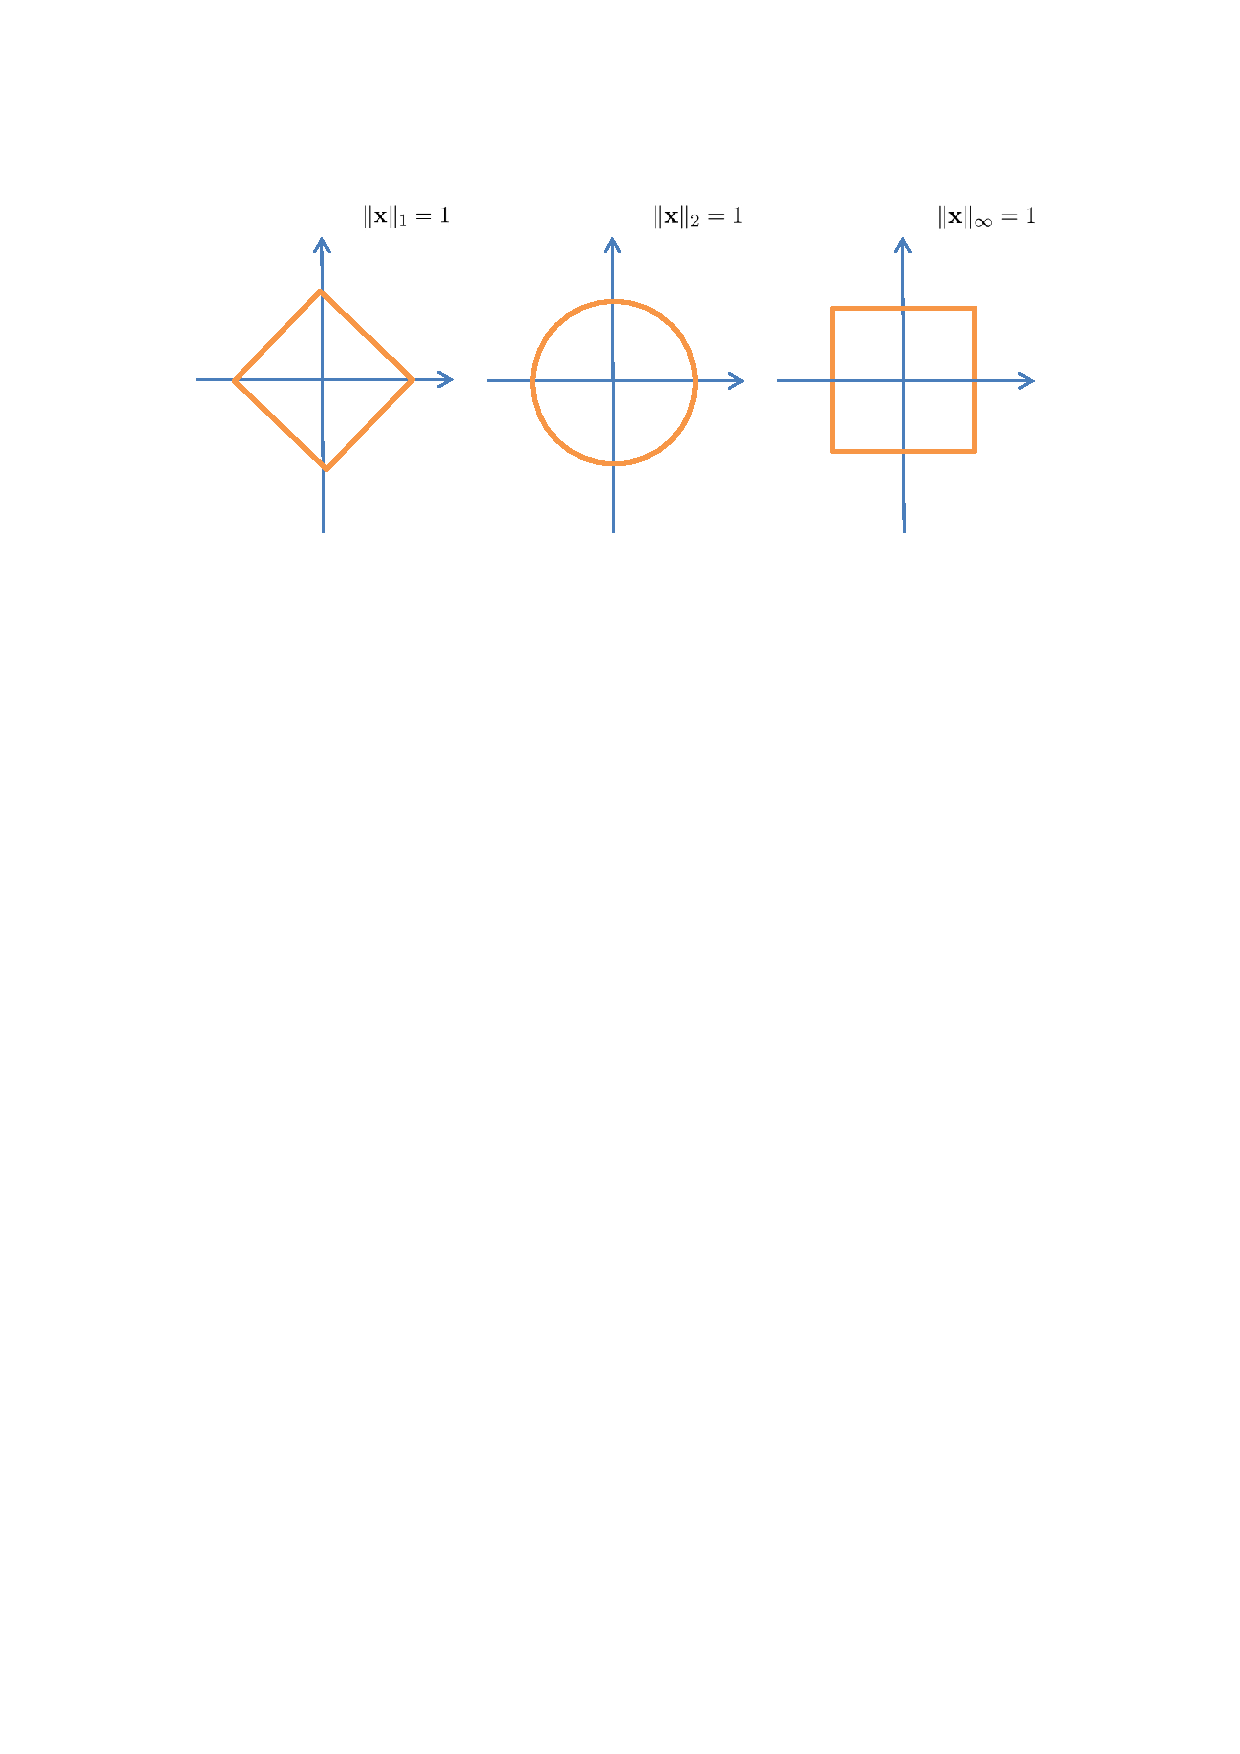
\includegraphics[width=0.9\textwidth]{norm.pdf}
\end{figure}

\end{document}



